\normaltrue \difficilefalse \tdifficilefalse
\correctionfalse

%\UPSTIidClasse{11} % 11 sup, 12 spé
%\newcommand{\UPSTIidClasse}{12}

\exer{Pompe à piston axial $\star$ \label{B2:13:PTSI:11}}
\setcounter{question}{0}\UPSTIcompetence[2]{B2-13}
\index{Compétence B2-13-PTSI}
\index{Pompe à piston axial}
\index{Arbre à cames}
\ifcorrection
\else
\marginnote{\textbf{Pas de corrigé pour cet exercice.}}
\fi

\ifprof
\else
Soit le mécanisme suivant. 
\begin{center}
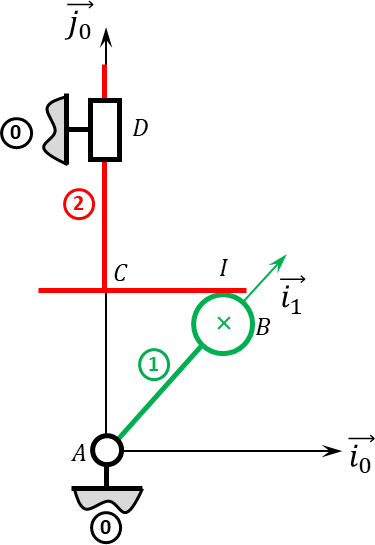
\includegraphics[width=.6\linewidth]{11_01}
\end{center}
\fi


\question{Réaliser le paramétrage du mécanisme.}
\ifprof
%$\torseurcin{V}{2}{0} = \torseurl{\vect{0}}{\lambdap (t)\vj{0}}{C}$.
\else
\fi



\ifprof
\else
\footnotesize
\ifcolle
\else

\fi
\normalsize
\begin{flushright}
\footnotesize{Corrigé  voir \ref{B2:13:PTSI:11}.}
\end{flushright}%
\fi